\chapter{Analyse van het probleem}
\label{Analyse_van_het_probleem}
%%%%%%%%%%%%%%%%%%%%%%%%%%%%%%%%%%%%%%%%%%%%%%%%%%%%%%%%%%%%%%%%%%%%%%%%

\begin{center}
    \begin{minipage}{0.5\textwidth}
        \begin{small}
            Waar de noodzaak van dit project word blootgelegd.
        \end{small} 
    \end{minipage}
    \vspace{0.5cm}
\end{center}

Kortweg is het probleem dat er momenteel niet met \ac{hdpe} en \ac{pp} kan
woorden ge-3D-print. 3D-printen met \ac{hdpe} en \ac{pp} is wenselijk omdat deze
materialen overvloedig zijn is de huidige afvalstroom, en ze dus goedkoop
te verkrijgen zijn.\\

Een voorbeeld van hoogwaardig PP in de afvalstroom zijn verpakkingen van
medische goederen in ziekenhuizen.  3devo heeft \ac{pp} bakjes van een
oogheelkunde kliniek en wil dat recyclen tot 3D-printer filament. Zie Figuur
\ref{fig:pp_bakjes} voor de bakjes.

\begin{figure}[h]
    \centerline{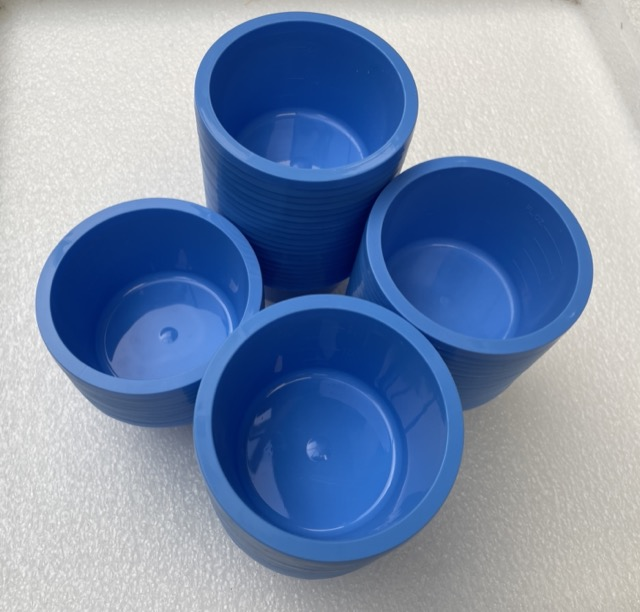
\includegraphics[width=0.4\textwidth]{pp_bakjes}}
    \caption{\ac{pp} bakjes van een oogheelkunde kliniek}
    \label{fig:pp_bakjes}
\end{figure}

%%%%%%%%%%%%%%%%%%%%%%%%%%%%%%%%%%%%%%%%%%%%%%%%%%%%%%%%%%%%%%%%%%%%%%%%
\section{Waarom is een speciale 3D-printer nodig}
%%%%%%%%%%%%%%%%%%%%%%%%%%%%%%%%%%%%%%%%%%%%%%%%%%%%%%%%%%%%%%%%%%%%%%%%

Er zijn twee redenen gegeven waarom een speciale printer nodig is voor het
printen met \ac{hdpe} en \ac{pp}.  Tests zijn uitgevoerd om vast te stellen of
deze complicaties werkelijk het printen van \ac{hdpe} en \ac{pp} onmogelijk
maken.

%%%%%%%%%%%%%%%%%%%%%%%%%%%%%%%%%%%%%%%%%%%%%%%%%%%%%%%%%%%%%%%%%%%%%%%%
\subsection{Printen op een conventionele 3D-printer}
%%%%%%%%%%%%%%%%%%%%%%%%%%%%%%%%%%%%%%%%%%%%%%%%%%%%%%%%%%%%%%%%%%%%%%%%

Er is een test uitgevoerd met het printen van \ac{hdpe} en \ac{pp}.  Deze test
zijn uitgevoerd op een conventionele \ac{fdm} 3D-printer, namelijk een Ender-3.
De slicer settings die gebruikt zijn waren vooral getweakt op temperatuur en
snelheid.

\begin{figure}[h]
    \centering
    \begin{minipage}{0.45\textwidth}
        \centerline{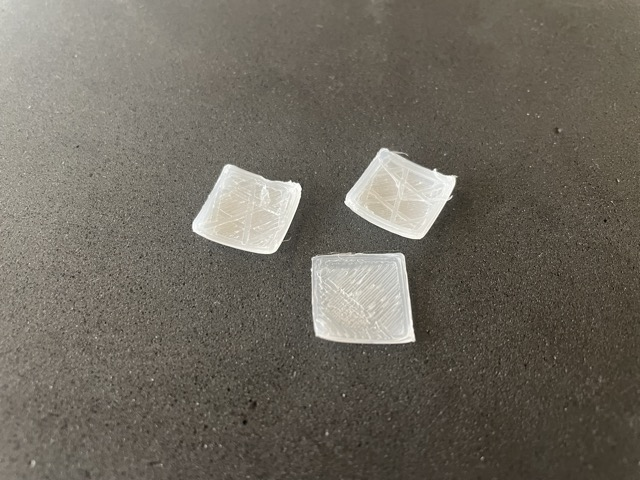
\includegraphics[width=0.9\textwidth]{hdpe_per_test}}
        \caption{Test print met \ac{hdpe} op een conventionele printer}
        \label{fig:hdpe_test}
    \end{minipage}\hfill
    \begin{minipage}{0.45\textwidth}
        \centerline{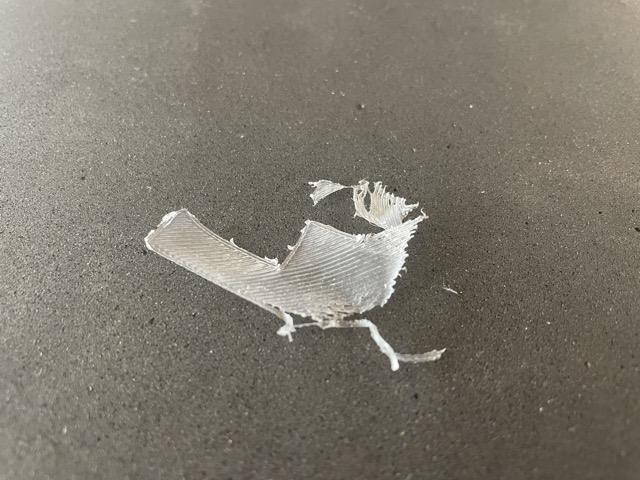
\includegraphics[width=0.9\textwidth]{pp_pre_test}}
        \caption{Test print met \ac{pp} op een conventionele printer}
        \label{fig:pp_test}
    \end{minipage}
\end{figure}

%%%%%%%%%%%%%%%%%%%%%%%%%%%%%%%%%%%%%%%%%%%%%%%%%%%%%%%%%%%%%%%%%%%%%%%%
\subsubsection{Laag hechting}
%%%%%%%%%%%%%%%%%%%%%%%%%%%%%%%%%%%%%%%%%%%%%%%%%%%%%%%%%%%%%%%%%%%%%%%%

De hypothese is dat bij het printen met \ac{pp} de laag hechting niet goed zal
zijn. Dat komt doordat \ac{pp} onder de kristallisatietemperatuur niet
''plakkerig'' is. De test met het printen van \ac{pp} heeft geconcludeerd dat
die hypothese waar is. Het materiaal blijft moeilijk plakken aan het bed, en als
dat goed ging, blijft het ook nauwelijks plakken aan zichzelf. Zie Figuur
\ref{fig:pp_test}. Een ander probleem met het printen van \ac{pp} is dat het
flexibele plastic niet goed door een bowden extruder gaat vanwege de extra
weerstand in dat systeem. Uitleg over wat een bowden tube extruder is staat in
hoofdstuk \ref{Bowden_extruder}. 

%%%%%%%%%%%%%%%%%%%%%%%%%%%%%%%%%%%%%%%%%%%%%%%%%%%%%%%%%%%%%%%%%%%%%%%%
\subsubsection{Krom trekken}
%%%%%%%%%%%%%%%%%%%%%%%%%%%%%%%%%%%%%%%%%%%%%%%%%%%%%%%%%%%%%%%%%%%%%%%%

De verwachting was dat het grote probleem met HDPE is dat het krom trekt tijdens
het printen. Tijdens het printen zal er een warmte gradiënt ontstaan, omdat de
laag die net is neergelegd al aan het afkoelen is voor dat de volgende de
volgende laag daar op word gelegd. Tijdens het testen op een conventionele
printer is vastgesteld dat dat inderdaad een probleem is, zie Figuur
\ref{fig:hdpe_test} voor een foto van de krom getrokken prints.

